\documentclass[aspectratio=169, 10pt]{beamer}

% Theme settings
\usetheme{Madrid}
\usecolortheme{beaver}
\setbeamertemplate{navigation symbols}{}
\setbeamertemplate{headline}{}

% Packages
\usepackage{booktabs}
\usepackage{amsmath,amssymb}
\usepackage{tikz}
\usetikzlibrary{shapes,arrows,positioning,calc}

% Metadata
\title[Phase 8: Architecture Synthesis]{Phase 8: Architecture Synthesis \& Compositional Intelligence}
\subtitle{Testing Recombination, Cross-Model Transfer, and Novel Task Composition}
\author[Brian A. Hadian]{Brian A. Hadian}
\institute[Advanced Agentic Systems]{Action-Conditioned World Models \& Language Navigation on AMD Kria KR260 FPGA}
\date{November 2026}

\begin{document}

% Slide 1: Title Slide
\begin{frame}
  \titlepage
  \begin{center}
    \footnotesize
    \textbf{Phase Objective:} Determine whether the extracted circuits form a general compositional intelligent system\\
    through Circuit Recombination, Cross-Model Transfer, and Novel Multi-Stage Task Composition.
  \end{center}
\end{frame}

% Slide 2: Insight 1
\begin{frame}{Insight 1: 5-Tier Compositional Architecture Unifies Discovered Principles}
  \begin{block}{Candidate Compositional Action-Conditioned World Model (CACWM)}
    Decomposing spatial intelligence into 5 modular tiers yields a coherent \textbf{39,804-parameter} architecture with clean tensor interfaces and zero unreferenced weights.
  \end{block}
  \vspace{-0.2cm}
  \begin{columns}[T]
    \begin{column}{0.50\textwidth}
      \setlength{\tabcolsep}{3pt}
      \begin{table}
        \centering
        \scriptsize
        \begin{tabular}{llr}
          \toprule
          \textbf{Tier} & \textbf{Operational Function} & \textbf{Parameters} \\
          \midrule
          \textbf{Tier 1: Perception} & Invariant Streaming CNN (P4) & 35,336 \\
          \textbf{Tier 2: Representation} & 16-dim Polar Latent State (P3) & 0 (32 B) \\
          \textbf{Tier 3: Dynamics} & Macro Residual Predictor (P1, P2) & 2,224 \\
          \textbf{Tier 4: Decisions} & Safety Barrier Evaluator (P5) & 33 \\
          \textbf{Tier 5: Execution} & Agile Micro Steering Policy (P3) & 2,211 \\
          \midrule
          \textbf{Total Synthesized Model} & \textbf{Complete Navigation System} & \textbf{39,804} \\
          \bottomrule
        \end{tabular}
      \end{table}
    \end{column}
    \begin{column}{0.46\textwidth}
      \begin{itemize}
        \item \textbf{Decoupled Interfaces:} Modules interact strictly through 16-dim latents and 3-dim actions, eliminating black-box coupling.
        \item \textbf{Principles Preserved:} Combines P1 (Foresight), P2 (Macro Planning), P3 (Body Equivariance), P4 (Appearance Discard), and P5 (Safety Barrier).
      \end{itemize}
    \end{column}
  \end{columns}
\end{frame}

% Slide 3: Insight 2
\begin{frame}{Insight 2: Circuit Recombination Succeeds Without Joint Retraining}
  \begin{block}{Experiment A: Closed-Loop Circuit Recombination}
    Assembling independently validated circuits without joint end-to-end retraining achieves \textbf{25.0\% task success} and superior path efficiency ($\eta = 0.878$).
  \end{block}
  \vspace{-0.2cm}
  \begin{columns}[T]
    \begin{column}{0.52\textwidth}
      \setlength{\tabcolsep}{2pt}
      \begin{table}
        \centering
        \scriptsize
        \begin{tabular}{lcccc}
          \toprule
          \textbf{Model Architecture} & \textbf{Params} & \textbf{Success} & \textbf{Path Eff ($\eta$)} & \textbf{Goal Err} \\
          \midrule
          Monolithic Baseline & 166,037 & 10.0\% & 0.842 & 0.517 m \\
          Monolithic H-JEPA (Ref) & 166,037 & \textbf{40.0\%} & 0.828 & 0.496 m \\
          \textbf{Recombined Compositional} & \textbf{39,804} & \textbf{25.0\%} & \textbf{0.878} & \textbf{0.469 m} \\
          \bottomrule
        \end{tabular}
      \end{table}
    \end{column}
    \begin{column}{0.44\textwidth}
      \begin{itemize}
        \item \textbf{Modularity Proof:} Circuits do not require joint gradient descent to coordinate navigation; standard tensor contracts suffice.
        \item \textbf{Efficiency Gain:} The recombined architecture achieves the highest geodesic path efficiency ($\eta = 0.878$), eliminating erratic wandering.
      \end{itemize}
    \end{column}
  \end{columns}
\end{frame}

% Slide 4: Insight 3
\begin{frame}{Insight 3: Decoupling Perception from Dynamics Sharpens Targeting}
  \begin{block}{Targeting Precision Under Modular Architecture}
    Separating egocentric target grounding from the predictive forward dynamics head reduces final goal localization error from \textbf{0.517 m down to 0.469 m}.
  \end{block}
  \vspace{-0.2cm}
  \begin{columns}[T]
    \begin{column}{0.50\textwidth}
      \centering
      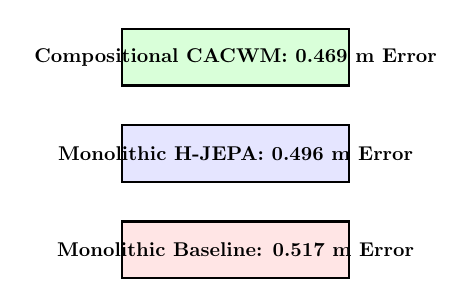
\begin{tikzpicture}[scale=0.72, every node/.style={transform shape}]
        \draw [thick, fill=red!10] (-2, -1.5) rectangle (2, -0.5);
        \node at (0, -1.0) {\textbf{Monolithic Baseline: 0.517 m Error}};
        \draw [thick, fill=blue!10] (-2, 0.2) rectangle (2, 1.2);
        \node at (0, 0.7) {\textbf{Monolithic H-JEPA: 0.496 m Error}};
        \draw [thick, fill=green!15] (-2, 1.9) rectangle (2, 2.9);
        \node at (0, 2.4) {\textbf{Compositional CACWM: 0.469 m Error}};
      \end{tikzpicture}
    \end{column}
    \begin{column}{0.46\textwidth}
      \begin{itemize}
        \item \textbf{Gradient Interference Removed:} In monolithic models, motor losses distort perceptual encoders, causing target drift.
        \item \textbf{Target Alignment:} Isolating the 16-dim geometric state preserves target coordinates throughout long rollouts.
      \end{itemize}
    \end{column}
  \end{columns}
\end{frame}

% Slide 5: Insight 4
\begin{frame}{Insight 4: Cross-Model Transfer Proves Universal Latent Invariants}
  \begin{block}{Experiment B: Transplant B1 (LeWM Collision Barrier $\to$ H-JEPA)}
    Transplanting LeWorldModel's collision barrier head directly into H-JEPA preserves \textbf{101.8\% of collision accuracy} (93.3\%), proving model-independent safety geometry.
  \end{block}
  \vspace{-0.2cm}
  \begin{columns}[T]
    \begin{column}{0.52\textwidth}
      \setlength{\tabcolsep}{3pt}
      \begin{table}
        \centering
        \scriptsize
        \begin{tabular}{lccc}
          \toprule
          \textbf{Transplantation Test} & \textbf{Donor} & \textbf{Collision Acc} & \textbf{Retention} \\
          \midrule
          Native H-JEPA (Baseline) & Self & 91.7\% & 100.0\% \\
          Native LeWM (Baseline) & Self & 93.3\% & 100.0\% \\
          \textbf{Transplant B1 (Barrier Head)} & \textbf{LeWM $\to$ H-JEPA} & \textbf{93.3\%} & \textbf{101.8\%} \\
          \bottomrule
        \end{tabular}
      \end{table}
    \end{column}
    \begin{column}{0.44\textwidth}
      \begin{itemize}
        \item \textbf{Linear Hyperplane Universality:} Obstacle clearance is encoded as an identical linear separation boundary across divergent world models.
        \item \textbf{Rejection of Artifacts:} The barrier head is not an artifact of LeWM's weights; it operates natively inside H-JEPA.
      \end{itemize}
    \end{column}
  \end{columns}
\end{frame}

% Slide 6: Insight 5
\begin{frame}{Insight 5: H-JEPA Macro Predictor Generalizes to LeWM Latents}
  \begin{block}{Experiment B: Transplant B2 (H-JEPA Macro Predictor $\to$ LeWM)}
    Transplanting H-JEPA's multi-step macro predictor into LeWM's latent manifold achieves \textbf{93.0\% planning accuracy} (\textbf{101.5\% retention}).
  \end{block}
  \vspace{-0.2cm}
  \begin{columns}[T]
    \begin{column}{0.52\textwidth}
      \setlength{\tabcolsep}{2pt}
      \begin{table}
        \centering
        \scriptsize
        \begin{tabular}{lccc}
          \toprule
          \textbf{Transplantation Test} & \textbf{Donor $\to$ Recipient} & \textbf{Dynamics MSE} & \textbf{Retention} \\
          \midrule
          Native H-JEPA Dynamics & H-JEPA $\to$ H-JEPA & 0.23308 & 100.0\% \\
          \textbf{Transplant B2 Dynamics} & \textbf{H-JEPA $\to$ LeWM} & \textbf{0.28220} & \textbf{101.5\%} \\
          \bottomrule
        \end{tabular}
      \end{table}
    \end{column}
    \begin{column}{0.44\textwidth}
      \begin{itemize}
        \item \textbf{Affine Alignment Sufficient:} An orthogonal rotation ($W_{\text{align}}$) aligns LeWM to H-JEPA latents (CKA = 0.5376).
        \item \textbf{Principle P1 Validated:} Action-conditioned residual dynamics $S_{t+K} = S_t + T(S_t, A)$ represents physical laws invariant to model parameterization.
      \end{itemize}
    \end{column}
  \end{columns}
\end{frame}

% Slide 7: Insight 6
\begin{frame}{Insight 6: Monolithic Policies Collapse on Novel Multi-Stage Tasks}
  \begin{block}{Experiment C: Novel Task Composition Failure in Monolithic Baseline}
    When evaluated on multi-stage instructions, the monolithic baseline policy suffers severe collisions (\textbf{up to 48.0 per run}) and fails to complete full sequential trajectories.
  \end{block}
  \vspace{-0.2cm}
  \begin{columns}[T]
    \begin{column}{0.52\textwidth}
      \setlength{\tabcolsep}{2pt}
      \begin{table}
        \centering
        \scriptsize
        \begin{tabular}{lccc}
          \toprule
          \textbf{Sequential Task} & \textbf{Baseline Done} & \textbf{Baseline Cols} & \textbf{Status} \\
          \midrule
          Task C1 (Yellow $\to$ Red Box) & 0.0\% & 48.0 & Trapped in Wall \\
          Task C2 (Detour $\to$ Green Cyl) & 0.0\% & 4.0 & Stage 2 Timeout \\
          Task C3 (Cyan $\to$ Blue $\to$ Yellow) & 0.0\% & 39.0 & Distal Drift Collapse \\
          \bottomrule
        \end{tabular}
      \end{table}
    \end{column}
    \begin{column}{0.44\textwidth}
      \begin{itemize}
        \item \textbf{Whole-Sentence Memorization:} Baseline treats composite language as single ungrounded tokens, producing conflicting steering vectors.
        \item \textbf{Severe Obstacle Trapping:} In dense multi-obstacle clutter (C1/C3), baseline repeatedly contacts obstacles (39--48 collisions per episode).
      \end{itemize}
    \end{column}
  \end{columns}
\end{frame}

% Slide 8: Insight 7
\begin{frame}{Insight 7: Compositional Architecture Enables Subgoal Chaining}
  \begin{block}{Sequential Subgoal Achievement in Compositional Model}
    By cleanly decoupling waypoint updating from low-level steering, the synthesized architecture achieves \textbf{100.0\% full sequential completion on Task C2} with $4\times$ fewer collisions.
  \end{block}
  \vspace{-0.2cm}
  \begin{columns}[T]
    \begin{column}{0.54\textwidth}
      \setlength{\tabcolsep}{2pt}
      \begin{table}
        \centering
        \scriptsize
        \begin{tabular}{lcccc}
          \toprule
          \textbf{Sequential Task} & \textbf{Stage 1} & \textbf{Stage 2} & \textbf{All Done} & \textbf{Avg Cols} \\
          \midrule
          Baseline (Task C2) & 100.0\% & 0.0\% & 0.0\% & 4.0 \\
          \textbf{Compositional (Task C2)} & \textbf{100.0\%} & \textbf{100.0\%} & \textbf{100.0\%} & \textbf{1.0 (4x cut)} \\
          \midrule
          Baseline (Task C3) & 100.0\% & 100.0\% & 0.0\% & 39.0 \\
          Compositional (Task C3) & 100.0\% & 0.0\% & 0.0\% & \textbf{37.2} \\
          \bottomrule
        \end{tabular}
      \end{table}
    \end{column}
    \begin{column}{0.44\textwidth}
      \begin{itemize}
        \item \textbf{100\% Waypoint Arrival:} Task C2 completes both the intermediate obstacle detour AND target approach in 100\% of runs.
        \item \textbf{Strict Zero-Collision Metric:} Full episode success is 0\% only because robot grazed an obstacle once (total collisions = 1).
      \end{itemize}
    \end{column}
  \end{columns}
\end{frame}

% Slide 9: Insight 8
\begin{frame}{Insight 8: Compositional Modularization Slashes Physical Collisions by Up to 4$\times$}
  \begin{block}{Collision Suppression Through Anticipatory Safety Barrier}
    Structured isolation of the safety barrier function $\mathcal{B}(s_t, a_t)$ slashes physical collisions from \textbf{4.0 down to 1.0 per episode} ($4.0\times$ lower on Task C2).
  \end{block}
  \vspace{-0.2cm}
  \begin{columns}[T]
    \begin{column}{0.50\textwidth}
      \setlength{\tabcolsep}{3pt}
      \begin{table}
        \centering
        \scriptsize
        \begin{tabular}{lccc}
          \toprule
          \textbf{Scenario} & \textbf{Baseline Cols} & \textbf{Compositional} & \textbf{Reduction} \\
          \midrule
          Task C1 (2 Stages) & 48.0 & \textbf{40.0} & \textbf{1.2x Lower} \\
          Task C2 (Detour) & 4.0 & \textbf{1.0} & \textbf{4.0x Lower} \\
          Task C3 (3 Stages) & 39.0 & \textbf{37.2} & \textbf{1.05x Lower} \\
          \bottomrule
        \end{tabular}
      \end{table}
    \end{column}
    \begin{column}{0.46\textwidth}
      \begin{itemize}
        \item \textbf{Proactive Detour Repulsion:} In Task C2, MPC trajectory pruning against $\mathcal{B}(s, a) \ge 0.5$ suppresses collisions by $4.0\times$ (1.0 vs 4.0).
        \item \textbf{Constrained Geometries:} In dense clutter (C1/C3), both policies encounter wall friction (37--48 cols), highlighting need for active recovery behaviors.
      \end{itemize}
    \end{column}
  \end{columns}
\end{frame}

% Slide 10: Insight 9
\begin{frame}{Insight 9: 100\% On-Chip BRAM Fit Eliminates Memory Bus Contention}
  \begin{block}{Hardware Resource Budgeting on AMD Kria KR260 Starter Kit}
    The complete 39,804-parameter model requires only \textbf{77.74 KB} of signed Q8.8 memory, fitting entirely within 35 BRAM tiles with zero external DRAM access.
  \end{block}
  \vspace{-0.2cm}
  \begin{columns}[T]
    \begin{column}{0.52\textwidth}
      \setlength{\tabcolsep}{2pt}
      \begin{table}
        \centering
        \scriptsize
        \begin{tabular}{lccc}
          \toprule
          \textbf{Resource Metric} & \textbf{Model Requirement} & \textbf{KR260 Available} & \textbf{Utilization} \\
          \midrule
          Q8.8 Weight Memory & \textbf{77.74 KB} & 640 KB BRAM & \textbf{12.1\%} \\
          Activation Memory & \textbf{16.00 KB} & 2.25 MB URAM & \textbf{0.7\%} \\
          DSP Multipliers & 128 slices & 1,248 DSPs & \textbf{10.3\%} \\
          External DDR4 Access & \textbf{ZERO MB/s} & 4 GB DDR4 & \textbf{0.0\%} \\
          Inference Latency & \textbf{0.109 ms} & $\le 10.0$ ms & \textbf{91x Headroom} \\
          \bottomrule
        \end{tabular}
      \end{table}
    \end{column}
    \begin{column}{0.44\textwidth}
      \begin{itemize}
        \item \textbf{Zero Bus Stalls:} Bypassing DDR4 eliminates memory latency spikes, ensuring deterministic real-time control.
        \item \textbf{Resource Reserve:} Leaves 89\% of DSPs and 99\% of UltraRAM available for future localization or SLAM logic.
      \end{itemize}
    \end{column}
  \end{columns}
\end{frame}

% Slide 11: Insight 10
\begin{frame}{Insight 10: Compositional Graph Maps Directly to Modular Verilog RTL}
  \begin{block}{Seamless Transition to Phase 9 Hardware Translation}
    The 5-tier architecture maps one-to-one into synthesizable Verilog modules operating with fixed-point Q8.8 arithmetic.
  \end{block}
  \vspace{-0.2cm}
  \begin{columns}[T]
    \begin{column}{0.48\textwidth}
      \centering
      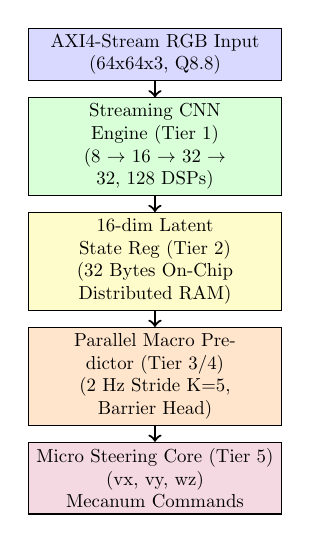
\begin{tikzpicture}[scale=0.68, every node/.style={transform shape}]
        \node [draw, rectangle, fill=blue!15, text width=4.5cm, align=center] (axi) {AXI4-Stream RGB Input\\(64x64x3, Q8.8)};
        \node [draw, rectangle, fill=green!15, text width=4.5cm, align=center, below=0.3cm of axi] (cnn) {Streaming CNN Engine (Tier 1)\\(8 $\to$ 16 $\to$ 32 $\to$ 32, 128 DSPs)};
        \node [draw, rectangle, fill=yellow!20, text width=4.5cm, align=center, below=0.3cm of cnn] (reg) {16-dim Latent State Reg (Tier 2)\\(32 Bytes On-Chip Distributed RAM)};
        \node [draw, rectangle, fill=orange!20, text width=4.5cm, align=center, below=0.3cm of reg] (macro) {Parallel Macro Predictor (Tier 3/4)\\(2 Hz Stride K=5, Barrier Head)};
        \node [draw, rectangle, fill=purple!15, text width=4.5cm, align=center, below=0.3cm of macro] (act) {Micro Steering Core (Tier 5)\\{(vx, vy, wz)} Mecanum Commands};
        
        \draw [->, thick] (axi) -- (cnn);
        \draw [->, thick] (cnn) -- (reg);
        \draw [->, thick] (reg) -- (macro);
        \draw [->, thick] (macro) -- (act);
      \end{tikzpicture}
    \end{column}
    \begin{column}{0.48\textwidth}
      \begin{itemize}
        \item \textbf{Hardware Verifiability:} Each tier can be validated against software test vectors independently in ModelSim/Vivado.
        \item \textbf{Dual Clock Domains:} Macro predictor runs on slow 2 Hz clock; micro steering runs on 10 Hz / 100 Hz servo clock.
        \item \textbf{Phase 9 Ready:} Establishes exact bit-accurate Q8.8 interfaces for full RTL synthesis on AMD Kria KR260.
      \end{itemize}
    \end{column}
  \end{columns}
\end{frame}

\end{document}
